\documentclass[letterpaper, 12pt]{article}
%
% This file contains configuration common to all guides.
% It is where all packages must be declared, along with project-wide configuration.
%

% No page numbering for individual guides -- overridden in cosig_full when compiling the entire project
\pagenumbering{gobble}

% Commands for the start of each guide
\newcommand{\cosigpart}[1]{
  \addcontentsline{toc}{part}{#1}
}
\newcommand{\cosigsection}[2]{
  \section*{#1}
  \phantomsection % avoid warnings from hyperref about the anchor of a bookmark and its parent's
  Last updated: #2 | \href{https://cosig.net}{cosig.net} | DOI: \href{https://doi.org/10.17605/OSF.IO/2KDEZ}{10.17605/OSF.IO/2KDEZ}
  \addcontentsline{toc}{section}{#1}
}

%
% Please keep the sections alphabetized by package name, unless a package needs to come first.
%

% Customize the table of contents
% Must come first or we get a "\@starttoc has already been redefined" warning and the package doesn't work
\usepackage{tocloft}

% Math environment + symbols
\usepackage{amsmath}
\usepackage{amssymb}

% Control caption layout
\usepackage[format=plain,labelfont={bf,it},textfont=it]{caption}
\captionsetup{justification=raggedright,singlelinecheck=false}

% Multi-line comments (via \begin{comment} ... \end{comment})
\usepackage{comment}

% Support for diacritics
\usepackage[T1]{fontenc} 

% Control page layout / margins
\usepackage{geometry}
\geometry{
    letterpaper,
    left=20mm,
    top=20mm,
    bottom=20mm
}

% More options for graphics
\usepackage{graphicx}

% Hyperlinks
\usepackage[hyperindex,breaklinks]{hyperref}
\hypersetup{
    colorlinks=true,
    linkcolor=blue,
    filecolor=magenta,      
    urlcolor=blue
}

% Code listings
\usepackage{listings}

% ORCID links
\usepackage{orcidlink}

% Improve paragraph spacing
\usepackage[skip=10pt plus1pt, indent=40pt]{parskip}

% LaTeX magic necessary for compilation
\usepackage{standalone}

% Document font, open alternative to Helvetica
\usepackage{tgheros}
\renewcommand{\familydefault}{\sfdefault}

% Control title layout
\usepackage{titlesec}
\titlespacing*{\section}{0pt}{1.5ex plus 1ex minus .2ex}{1.3ex plus .2ex}

\begin{document}
\flushleft\includegraphics[width=0.5\textwidth]{img/home/241017_final_logo_mockup.png}

\cosigsection{Magnetometry}{3 November 2026}

In materials science, magnetometry typically describes the process of measuing a sample's total \href{https://en.wikipedia.org/wiki/Magnetic_moment}{magnetic moment} $m_\text{total}$. These samples can come in many forms, including bulk materials like pellets, powders and single crystals as well as magnetic thin films that are deposited on various substrates. As $m_\text{total}$ also depends on the sample volume, most results report in magnetization $M$, which describes total magnetic moment per unit volume. $m_\text{total}$ arises from the vector sum of individual magnetic moments, inlcuding electron spin and orbital moments $\mu_i$. In equation form, $M$ is thus expressed as 

$$
M = \frac{1}{V}\sum_{i}\mu_i = \frac{m_\text{total}}{V},
$$

where V is the sample volume.

Note that while M is a vector in three-dimensional space (each individual component $\mu_i$ is itself a vector, for magnetometry purposes, it is typically conceptualized as the magnitude of that vector along a particular axis.

Magnetometry typically involves obtaining a magnetization-magnetic field curve (or M-H curve). M-H curves how the magnetization of a sample $M$ changes in response to an externally-applied magnetic field $H$. M-H curves are typically recorded using a \href{https://en.wikipedia.org/wiki/Vibrating-sample_magnetometer}{vibrating sample magnetometer (VSM)} or a \href{https://en.wikipedia.org/wiki/SQUID}{superconducting quantum interference device (SQUID)}-based magnetic property measurement system (MPMS). 

\subsection*{Paramagnetic and diamagnetic materials}

How a material behaves under the M-H curve is determined by its magnetic susceptibility $\chi_m$. Some materials may be characterized by a constant $\chi_m$ at a fixed temperature. For these materials, the M-H curves are approximated using a simple linear function such that

$$M = \chi_m H,$$

where $H$ is the external magnetic field. Materials with a constant positive susceptibility ($\chi_m > 0$, i.e., materials that produce a weak magnetization in the same direction as the applied magnetic field) are classified as \href{https://en.wikipedia.org/wiki/Paramagnetism}{paramagnetic} materials. Materials with a constant negative susceptibility ($\chi_m < 0$, i.e., materials that produce a weak magnetization in the opposite direction as the applied magnetic field) are classified as \href{https://en.wikipedia.org/wiki/Diamagnetism}{diamagnetic} materials. Because they do not interact very strongly with a permanent magnet, both paramagnetic materials (e.g., aluminum and titanium) and diamagnetic materials (e.g., gold and water) are commonly, but inaccurately, referred to as ``non-magnetic''. In paramagnetic and diamagnetic materials, the magnetization induced by the external magnetic field is not permanent; as soon as the external magnetic field is removed, the material’s magnetization also goes away (notice that by the previous equation, $H = 0$ implies $M = 0$).

\subsection*{Ferromagnetic and ferrimagnetic systems}

Other classes of materials, such as \href{https://en.wikipedia.org/wiki/Ferromagnetism}{ferromagnetic} and \href{https://en.wikipedia.org/wiki/Ferrimagnetism}{ferrimagnetic} materials, exhibit more complex M-H curves. Unlike paramagnetic and diamagnetic materials, the magnetic susceptibilities $\chi_m(H)$ of these materials vary with the magnetic field (but remain positive, similar to paramagnetic materials). In ferromagnetic and ferrimagnetic materials, $M$ is typically much larger in magnitude than for paramagnetic and diamagnetic materials. These materials undergo \href{https://en.wikipedia.org/wiki/Magnetic_hysteresis}{magnetic hysteresis}: when the external magnetic field is removed, part of the material’s magnetization remains.

For ferromagnetic materials (e.g., iron), most of the magnetic moments align with the field-axis when the external magnetic field is set beyond a certain field strength known as the saturating field ($H_\text{sat}$). At this point, the material reaches its maximum magnetization (i.e., its saturation magnetization $M_s$). Ferrimagnetic materials also respond strongly to an external magnetic field and share the same M-H curve features as ferromagnetic materials. However, the atoms of ferrimagnets (e.g., magnetite) are arranged in at least two sublattices with opposing, but unequal magnetic moments such that the net total magnetic moment of the material is still positive. As such, ferrimagnets typically produce lower magnetization than ferromagnets.

When carrying out magnetometry on ferromagnetic or ferrimagnetic materials, the sample is first subjected to a large magnetic field along the field axis to saturate the magnetization within the sample. The field is swept from one saturating field ($H_\text{sat}$) to the other ($-H_\text{sat}$) and then swept again in reverse to form what is known as a hysteresis loop. There are three magnetic parameters that characterize the hysteresis loop: saturation magnetization, remanent magnetization and intrinsic coercivity.

\begin{itemize}
    \setlength\itemsep{-0.5em}
    \item \emph{Saturation magnetization} $M_s$ is defined as the maximum magnetization a material can attain. $M_s$ is typically expressed in units of amperes per cubic meter (A/m, \href{https://en.wikipedia.org/wiki/International_System_of_Units}{SI units}) or electromagnetic units per cubic centimeter (EMU/cc or EMU/cm$^3$, \href{https://en.wikipedia.org/wiki/Centimetre%E2%80%93gram%E2%80%93second_system_of_units}{CGS units}). Many studies on bulk materials also report mass-specific saturation magnetization in electromagnetic units per gram (EMU/g, CGS units). $M_s$ is derived from an M-H curve by taking the constant magnitude of $M$ from either end of the hysteresis cruve. At these large fields, most of the magnetic moments within a ferromagnetic sample are aligned in the same direction as the field. For a ferrimagnetic sample, most of the magnetic moments are aligned collinear (parallel or antiparallel) to the field direction.
    \item \emph{Remanent magnetization} $M_r$ is defined as the magnetization remaining at zero field in the hysteresis lop. It measures the sample's ability to retain its magnetization in the absence of any external field. For example, a hard permanent magnet such as \href{https://en.wikipedia.org/wiki/Neodymium_magnet}{NbFeB} is characterized by large $M_r$ since it can retain most of its magnetization. In contrast, a soft magnet (e.g., \href{https://en.wikipedia.org/wiki/Ferrite_(magnet)}{ferrites} including Mn-Zn, Ni-Zn) loses nearly all of its magnetization once the external field is removed. The measure of \emph{squareness} $S = \frac{M_r}{M_s}$ quantifies the rectangular appearance of the M-H curve. A maximum $S = 1$ indicates a perfectly rectangular hysteresis loop.
    \item \emph{Instrinsic coercivity} $H_c$ or $H_{ci}$ is defined as the magnetic field $H$ at which the M-H curve crosses $M = 0$. This means that when $H = H_c$, all magnetic moments in the sample sum to zero. Qualitatively, coercivity is a measure of how resistant the sample is to switching its magnetization. A high coercivity represents a stronger resistance to switching since a larger field is required to switch at least half of the total magnetic moments. $H_c$ is expressed in units of oersted (Oe, CGS units) or Tesla (T, SI units).  
\end{itemize}

\begin{figure}[h!tbp]
    \centering
    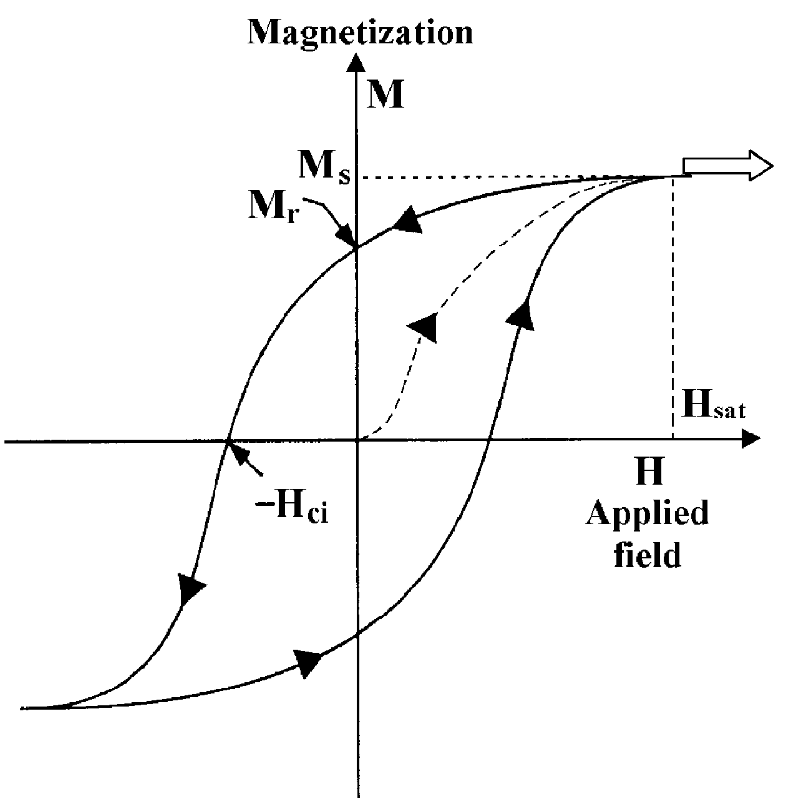
\includegraphics[width=0.8\textwidth]{img/magnetometry/sung_rudowicz_1a.png}
    \caption*{Standard magnetic hysteresis loop. The dashed line leading from the origin to the top right corner of the hysteresis loop is known as the initial magnetization curve and describes the material's behavior before external magnetic field sweeping begins. Adapted from \href{https://doi.org/10.1016/S0304-8853(02)01339-2}{Sung and Rudowicz (2003)}.}
\end{figure}

\subsection*{M-H curves versus B-H curves}

The M-H curve (or magnetization curve) is closely related to but distinct from the B-H curve (or magnetic induction/magnetic flux density curve). While $M$ denotes the total magnetization (per unit volume), $B$ represents the total magnetic field intensity inside the sample (attributable both to the sample’s magnetization M as well as the external magnetic field $H$). $B$ is related to $M$ by 

$$B = \mu_0 (M + H)$$ 

where $\mu_0$ is the \href{https://en.wikipedia.org/wiki/Vacuum_permeability}{permeability of free space}.

M-H curves and B-H curves are often confused. As stated by \href{https://doi.org/10.1016/S0304-8853(02)01339-2}{Sung and Rudowicz (2003)}:

\begin{quote}
    \textit{Both curves B vs. H and M vs. H have similar general characteristics, except for one crucial point. After the saturation point is reached, the M vs. H curve becomes a straight line with exactly zero slope, whereas the slope of the B vs. H curve reflects the constant magnetic susceptibility. In other words, the B vs. H curve does not saturate by approaching a limiting value as in the case of the M vs. H curve.}
\end{quote}

\pagebreak

\subsection*{Example 1: Correct interpretation of hysteresis loop}

\href{https://doi.org/10.1063/1.4979921}{Li et al. (2017)} perform magnetometry on La$_0.7$Sr$_0.3$CoO$_3$ grown on (LaAlO$_3$)$_{0.3}$(Sr$_2$AlTaO$_6$)$_{0.7}$ subtrates with various thicknesses (4, 8 and 12 nm). The authors report $M_s$ and $M_r$ for 8 and 12 nm:

\begin{quote}
    \textit{The saturation magnetization ($M_s$) for sample C12 ($\sim$ 150 emu/cm$^3$) is close to that of the bulk LSCO, while it decreases to 125 emu/cm$^3$ when the thickness is reduced to 8 nm. At the same time, the coercive field decreases from 0.90 T to 0.72 T...}
\end{quote}

Note that:

\begin{itemize}
    \setlength\itemsep{-0.5em}
    \item Magnetic saturation is observed in the hysteresis loops for 8 and 12 nm (C8 and C12). $M$ is relatively constant at both ends of the hysteresis loops. $M_s$ can be accurately extracted.
    \item The reported $M_s$ values of 150 and 125 emu/cc are consistent with the maximum $M$ at the ends of the hysteresis loops for C12 and C8, respectively. 
    \item The reported $H_c$ values of $0.9$ and $0.72$ T are also consistent with $H(M=0)$ of the hysteresis loops for C12 and C8, respectively.
\end{itemize}

\begin{figure}[h!tbp]
    \centering
    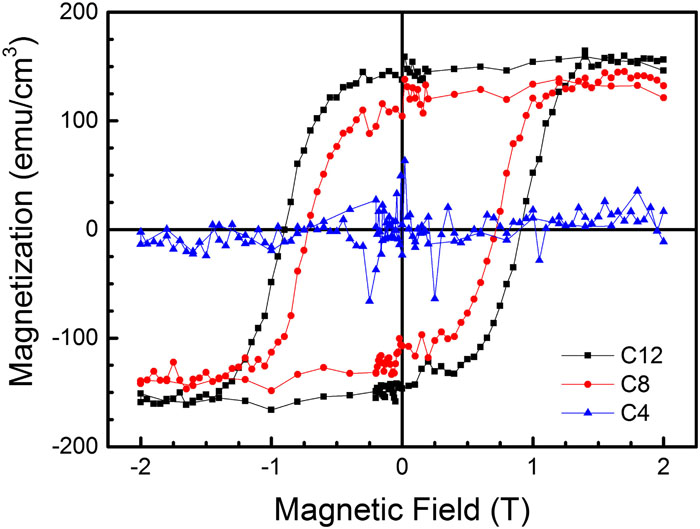
\includegraphics[width=0.8\textwidth]{img/magnetometry/045003_1_f3.jpeg}
    \caption*{Magnetic hysteresis loops for La$_0.7$Sr$_0.3$CoO$_3$ of various thicknesses obtained using SQUID magnetometry. Adapted from \href{https://doi.org/10.1063/1.4979921}{Li et al. (2017).}}
\end{figure}

\pagebreak

\subsection*{Example 2: Inappropriate measurement of $M_s$}

\href{https://doi.org/10.1016/j.ceramint.2024.08.126}{Khan et al. (2024)} claim to measure $M_s$ of ``3\% Cr doped ZnO'' (CZ-B) and ``4.5\% Cr doped ZnO'' (CZ-C) nanoparticles using VSM. However, the hysteresis loop for CZ-C does not appear to display constant saturation magnetization at large fields (indicated by the nonzero slope in the green dashed circle in the figure below). Nonetheless, they reported $M_s$ as 33.17 memu/g. The authors appear to have taken the maximum M at the largest field from a hysteresis curve that does not show any magnetic saturation. This interpretation of $M_s$ is inappropriate.

\begin{figure}[h!tbp]
    \centering
    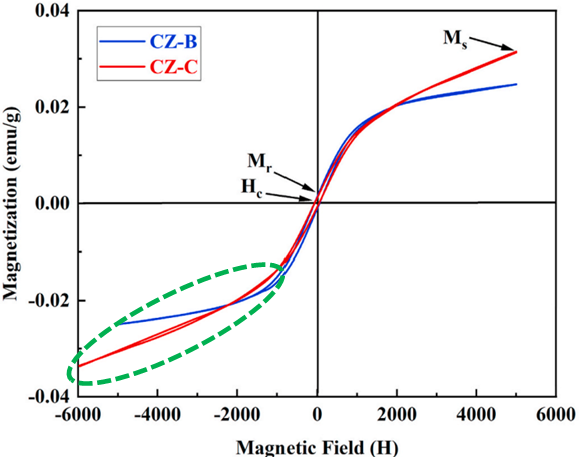
\includegraphics[width=0.8\textwidth]{img/magnetometry/image-1756723730188.png}
    \caption*{Problematic M-H loop, adapted from \href{https://doi.org/10.1016/j.ceramint.2024.08.126}{Khan et al. (2024)} by \href{https://pubpeer.com/publications/22EC374C59A3360135B89E22C62AD3\#4}{Jian Peng Chan on PubPeer}.}
\end{figure}

\pagebreak

\subsection*{Example 3: Innapropriate measurement of $M_s$}

In \href{https://doi.org/10.1016/j.jallcom.2016.05.043}{Birajdar et al. (2016)}, the authors extract Ms from the M-H curves obtained from Zn$_{1-x}$Co$_{x}$O nanoparticles at various Co concentrations. However, most of the M-H curves display either linear paramagnetic behavior or were measured with fields that were insufficient to achieve magnetic saturation. Here, the authors extracted $M_s$ by taking the maximum magnetization at each end of M-H curves that do not display magnetic saturation.

\begin{figure}[h!tbp]
    \centering
    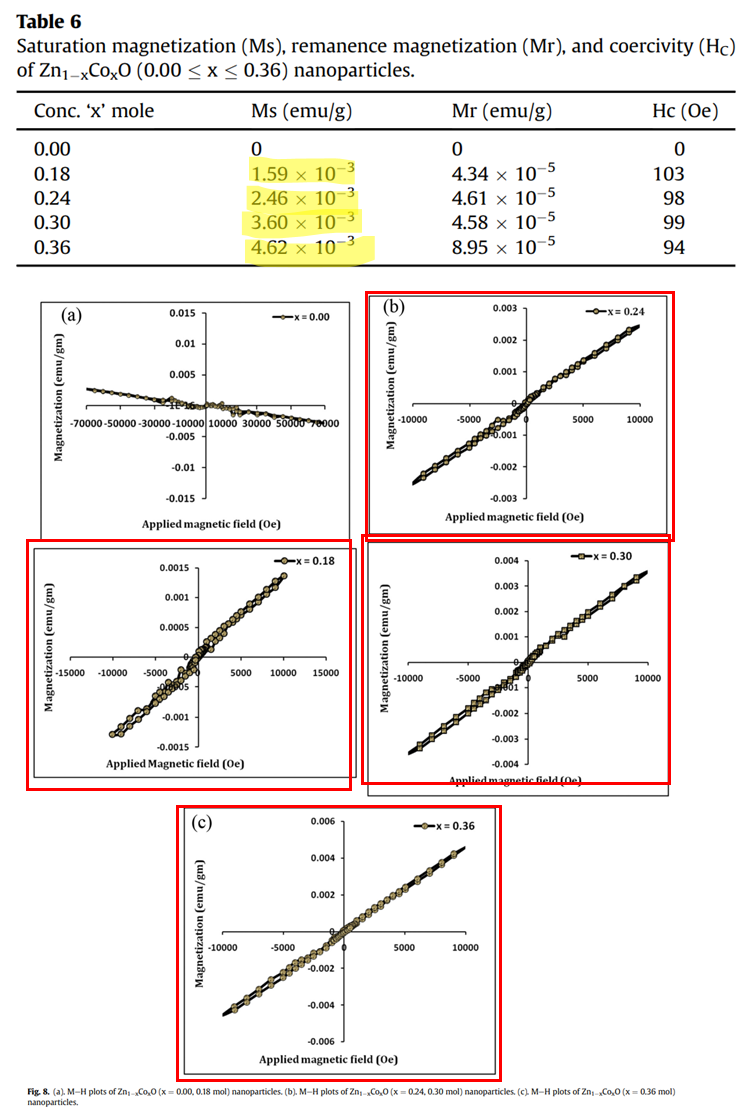
\includegraphics[width=0.7\textwidth]{img/magnetometry/image-1756726251008.png}
    \caption*{Problematic M-H curves, adapted from \href{https://doi.org/10.1016/j.jallcom.2016.05.043}{Birajdar et al. (2016)} by \href{https://pubpeer.com/publications/ED0909327637962263A3F2E265F1B0\#6}{Jian Peng Chan on PubPeer}.}
\end{figure}

\pagebreak

\subsection*{Example 4: Non-corresponding magnetic parameters}

Irregularities can often be spotted by simply exercising the definitions of common hysteresis parameters including $H_c$, $M_r$ and $M_s$. 

\href{https://doi.org/10.1007/s10854-023-10200-8}{Ibrahim et al. (2023)} report the M-H curves obtained through room-temperature VSM conducted on LaFe$_{1-x}$Cr$_x$O$_3$ perovskites (where $x$ = 0, 0.1, 0.2, 0.3, 0.4, 0.5). The authors outline the three major parameters in Table 3, but many of these values do not correspond to the M-H loops in the authors’ Figure 12. Irregularities in the table include:

\begin{itemize}
    \setlength\itemsep{-0.5em}
    \item Inappropriate attribution of $M_s$ to M-H loops exhibiting linear paramagnetic behavior (red underline). No magnetic saturation is observed in these M-H curves.
    \item $M_r$ beyond the range of the vertical axis.
    \item $M_r \gg M_s$ leading to $R > 1.0$, which is not possible.
    \item Inconsistent $H_c$ for LaFeO$_3$. The inset in Figure 12 does not appear to show $M = 0$ at 1020 Oe (black underline). Based on their respective M-H curves, coercivities for all specimens are significantly less than 1 kOe.
\end{itemize}

\begin{figure}[h!tbp]
    \centering
    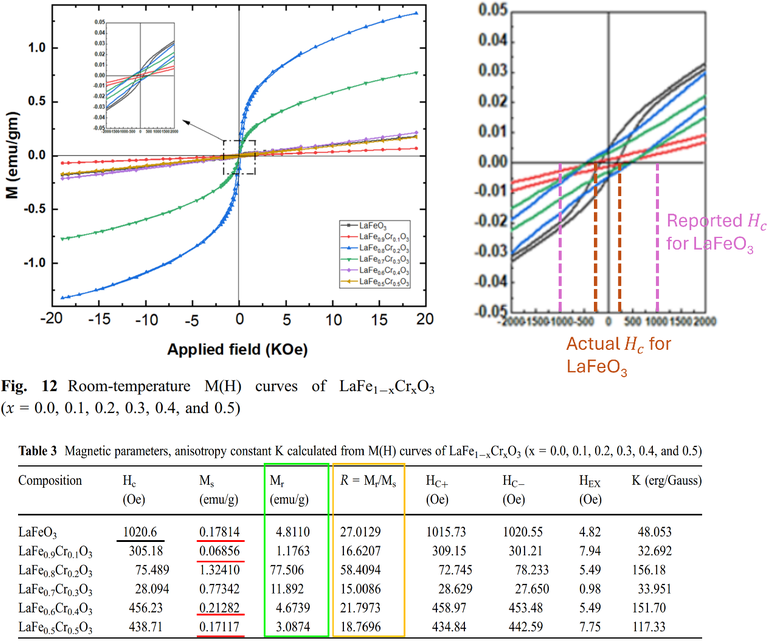
\includegraphics[width=0.9\textwidth]{img/magnetometry/ibrahim_et_al_explanation.png}
    \caption*{Problematic table of magnetic parameters and corresponding M-H curves. Adapted from \href{https://doi.org/10.1007/s10854-023-10200-8}{Ibrahim et al. (2023)}.}
\end{figure}

\subsection*{Example 5: Non-corresponding magnetic parameters}

In \href{https://doi.org/10.1016/j.molstruc.2022.133289}{Kanithan et al. (2022)}, the results shown for hysteresis obtained via VSM carried out on Mg$^{2+}$-doped NiFe$_2$O$_4$ contain several discrepancies between figures and tables. In particular,

\begin{itemize}
    \setlength\itemsep{-0.5em}
    \item For all fractions of Mg$^{2+}$, all $M_s$ values shown in Table 2 are much smaller than the $M_s$ values that can be estimated from Figure 8.
    \item The $M_r$ values shown in Table 2 are much larger than the $M_r$ values that can estimated from Figure 8. 
\end{itemize}

\begin{figure}[h!tbp]
    \centering
    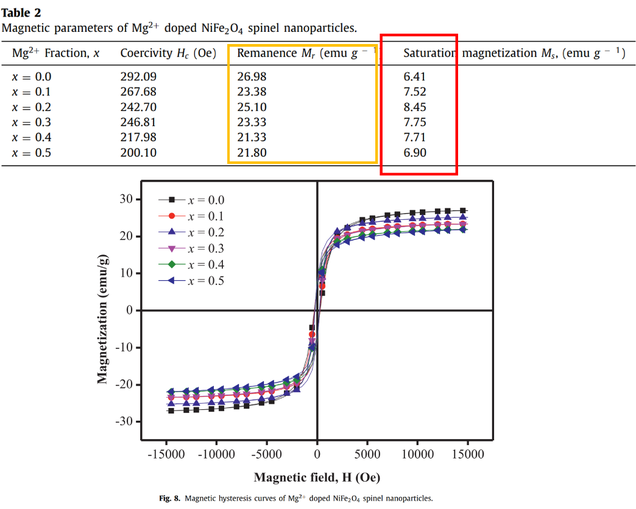
\includegraphics[width=0.9\textwidth]{img/magnetometry/kanithan_et_al_explanation.png}
    \caption*{Problematic table of magnetic parameters and corresponding M-H curves. Adapted from \href{https://doi.org/10.1016/j.molstruc.2022.133289}{Kanithan et al. (2022)}.}
\end{figure}

\subsection*{Additional resources}

\begin{itemize}
    \setlength\itemsep{-0.5em}
    \item \href{https://doi.org/10.1016/S0304-8853(02)01339-2}{``Physics behind the magnetic hysteresis loop—a survey of misconceptions in magnetism literature'' (2003)}
    \item \href{https://msestudent.com/b-h-vs-m-h-hysteresis-loops-magnetic-induction-vs-magnetization-similarities-differences-and-points-on-the-graph/}{``B-H vs M-H Hysteresis Loops: Magnetic Induction vs Magnetization (Similarities, Differences, and Points on the Graph)'' (2020)}
\end{itemize}

\end{document}